\documentclass[12pt]{article}

\usepackage{algorithmic}
\usepackage{amsmath}
\usepackage{graphicx}
\usepackage{hyperref}
\usepackage{booktabs}

\begin{document}

\title{CSI709 Midterm \\
Problem 1}
\author{
        Geoffrey Ulman \\
        George Mason University\\
}
\date{\today}

\maketitle

\section{K-Means Clustering}

The results of the k-means clustering performed on 84 samples of fiduciary point data (after centering the data and calculating \(dx\) and \(dy\) offsets from the average centered grid) is included in Table \ref{gini}.

\begin{table}\scriptsize
\begin{center}
\caption{Contents and Gini Index of K-Means Clusters}
\begin{tabular}{lr}
\\
\toprule
Cluster & Gini Index \\
\midrule
fjem0,fjem0,fjem0,fjem0 & 0.000 \\ \midrule
fadg0,fadg0 & 0.000 \\ \midrule
mstk0,mgwt0 & 0.500 \\ \midrule
fadg0,fedw0,fedw0 & \\
fedw0,fjem0,mpgl0 & 0.667 \\ \midrule
mtmr0,mtmr0,mtmr0 & \\
mtmr0,mtmr0,mdab0 & 0.278 \\ \midrule
mrjo0,mrjo0,mrjo0 & 0.000 \\ \midrule
mwbt0,mwbt0,mwbt0 & \\
mwbt0,msjs1 & 0.320 \\ \midrule
mrcz0,mrcz0,mrcz0,mrcz0 & \\
mrcz0,fedw0,mmdm2,mreb0 & \\
mreb0,mreb0,mreb0 & 0.645 \\ \midrule
fadg0,fadg0 & 0.000 \\ \midrule
mstk0,mdld0 & 0.500 \\ \midrule
fram1,fram1,fram1 & \\
fram1,fram1 & 0.000 \\ \midrule
mgwt0,mgwt0,mgwt0 & \\
mwbt0,mdab0 & 0.560 \\ \midrule
mstk0,mstk0 & 0.000 \\ \midrule
mrjo0,mreb0 & 0.500 \\ \midrule
msjs1,msjs1 & 0.000 \\ \midrule
fkms0,fpkt0,fpkt0 & \\
fpkt0,fpkt0, & 0.320 \\ \midrule
mdld0,mdld0,mdld0 & 0.000 \\ \midrule
mtas1,mtas1,mdab0 & \\
mdab0,mdld0 & 0.640 \\ \midrule
mcem0,mcem0,mcem0,mcem0 & \\
fkms0,fkms0,mtas1,mtas1 & 0.625 \\ \midrule
mmdm2,mmdm2,mmdm2,mmdm2 & 0.000 \\
\bottomrule
\end{tabular}
\end{center}
\end{table}
\label{gini}

\begin{figure}
\centering
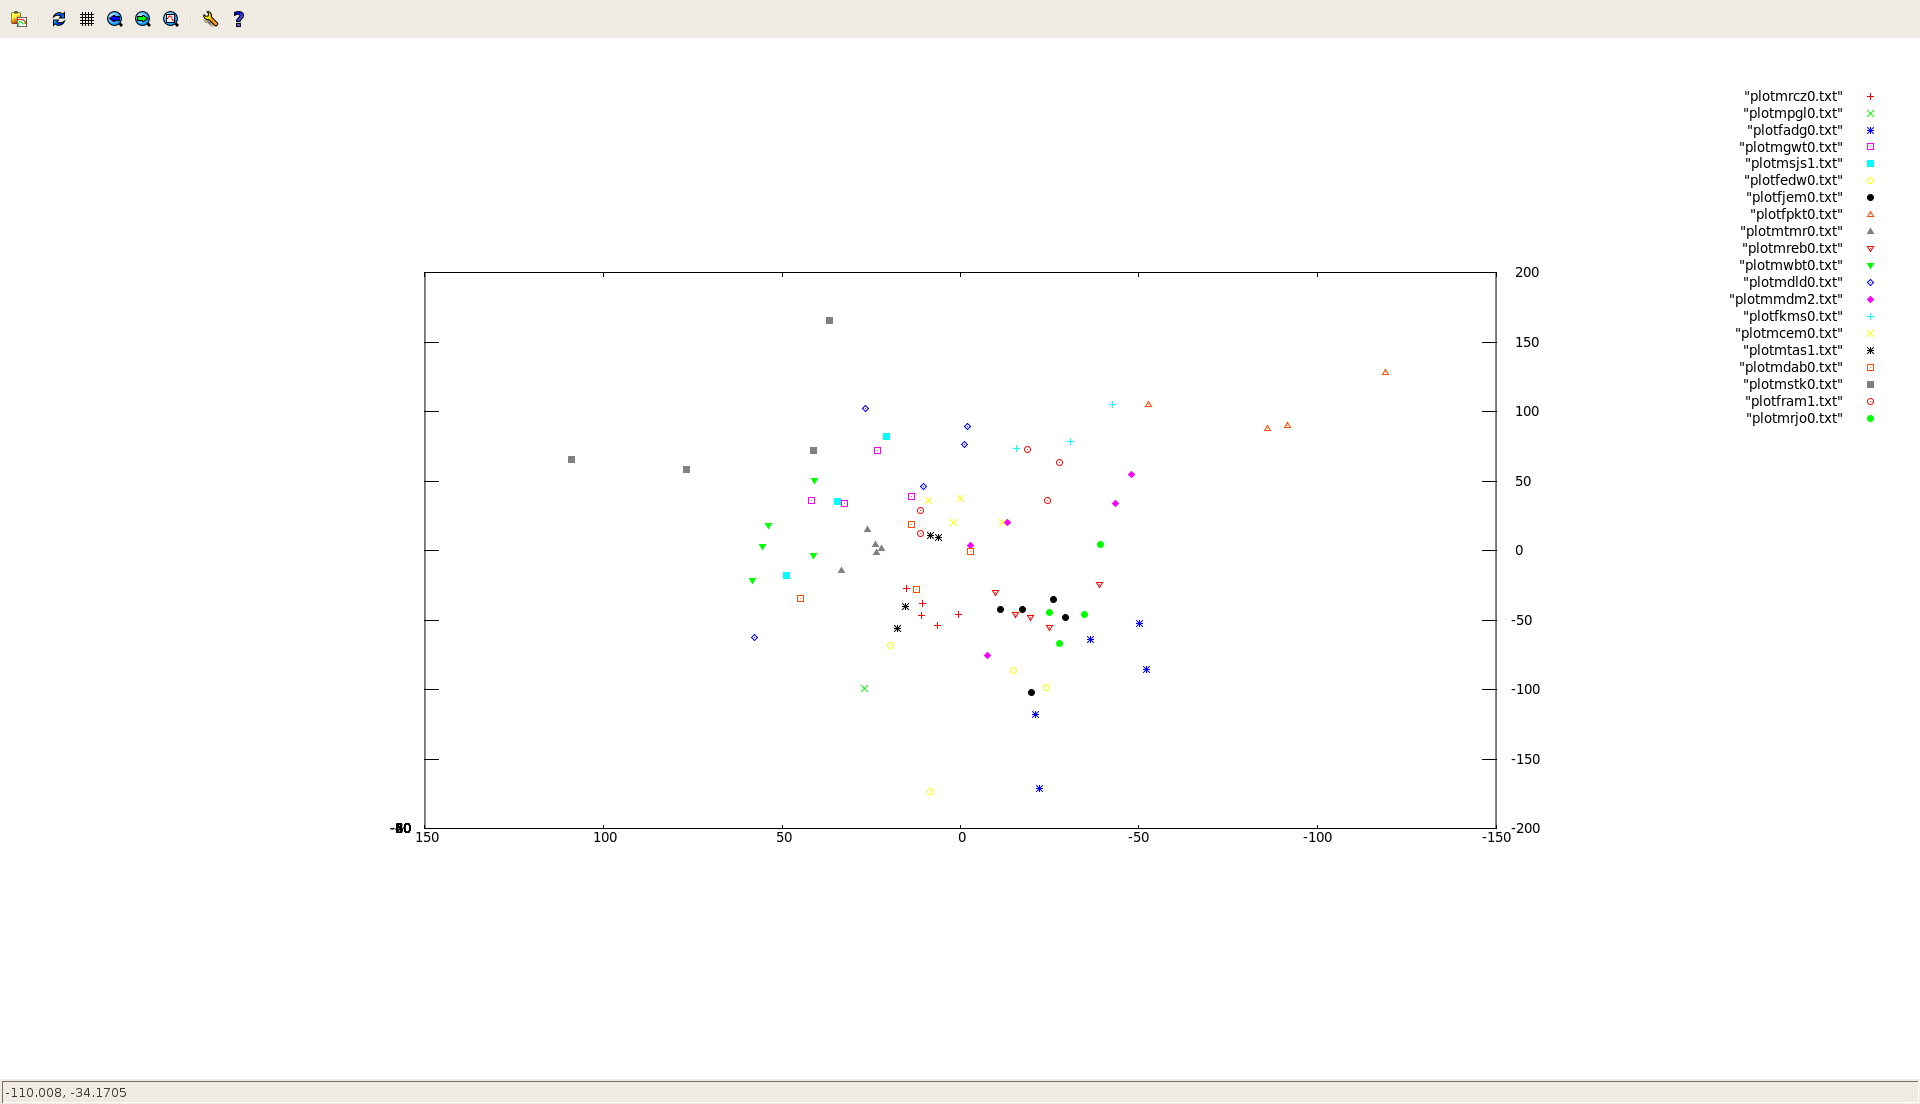
\includegraphics[width=0.30\textwidth]{problem1-fid-pca-1.png}
\caption{Fiduciary Point Offsets In PCA Space}
\label{pca1}
\end{figure}

\begin{figure}
\centering
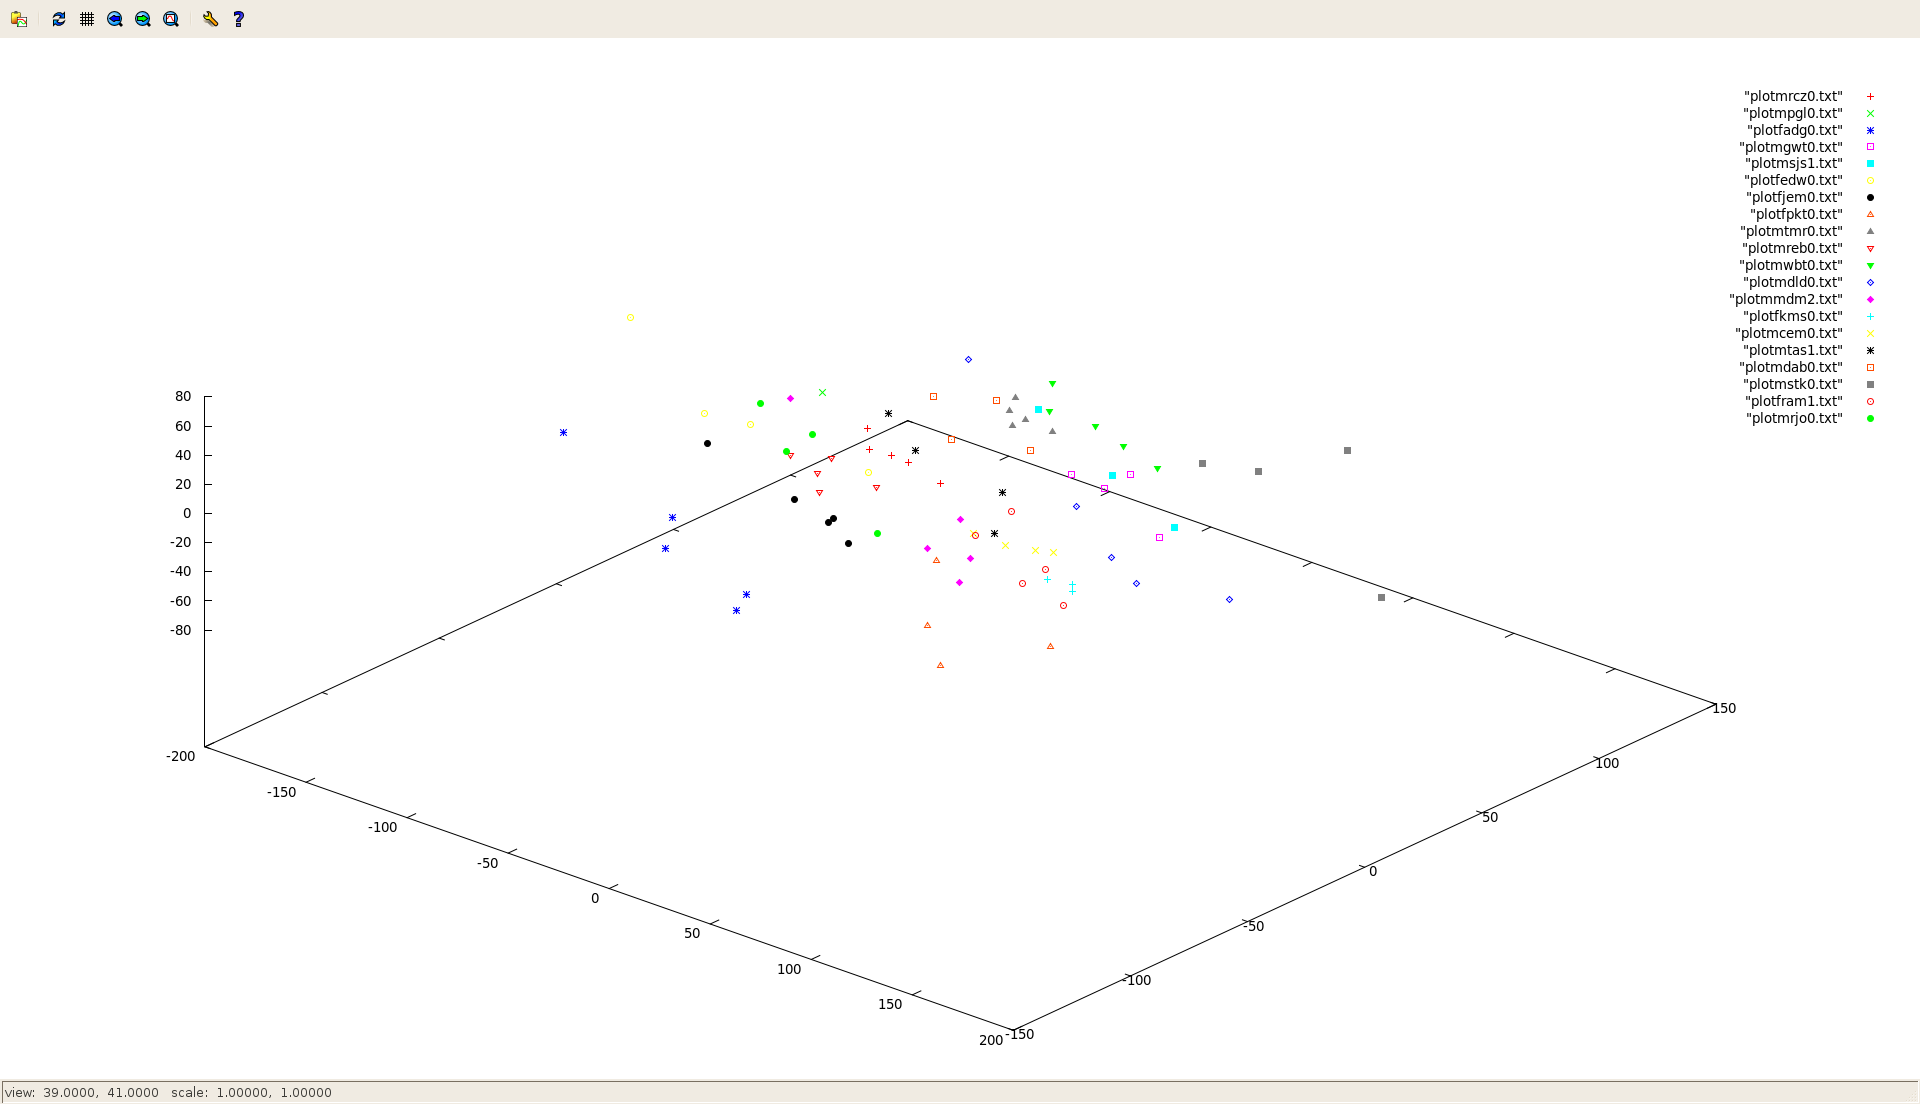
\includegraphics[width=0.30\textwidth]{problem1-fid-pca-2.png}
\caption{Fiduciary Point Offsets In PCA Space (Rotated View)}
\label{pca2}
\end{figure}

\end{document}
